%%%%%%%%%%%%%%%%%%%%%%%%%%%%%%%%%%%%%%%%%%%%%%%%%%%%%%%%%%%%%%%%%%%%%%%%%%%%%%%
%  s04a-fukaya.tex —— 第 4 节 The Fukaya category（§4.1–§4.4）
%  原文：Ivan Smith, \emph{A Symplectic Prolegomenon}, arXiv:1401.0269v2
%        源码第 963–1164 行（原文第 24–29 页）
%  说明：本节只含 §4 的前半部分；§4.5 起由 s04b-fukaya.tex 接续。
%%%%%%%%%%%%%%%%%%%%%%%%%%%%%%%%%%%%%%%%%%%%%%%%%%%%%%%%%%%%%%%%%%%%%%%%%%%%%%%

\section{Fukaya 范畴}\label{Sec:Fukaya}

\begin{keypoints}
\begin{itemize}
  \item \textbf{核心图像}：Fukaya 范畴 $\scrF(X)$ 以恰当或单调的拉格朗日子流形为对象、以 Floer 上同调群为态射空间，并用全纯圆盘的计数定义 $A_{\infty}$ 复合；它是拉格朗日相交数理论的范畴化。
  \item \textbf{关键工具}：$A_{\infty}$ 关系的树图（mangrove）表述、Stasheff 结合面体与 Deligne--Mumford 紧化、扭曲复形与幂等完备化。
  \item \textbf{结构结论}：链水平的 $\mu^2$ 只结合到同伦，高阶运算 $\mu^d$（$d\ge 3$）不是链映射、也不下传到上同调；只有在 $H(\scrA)$ 上才恢复通常的范畴结构。
  \item \textbf{三角结构}：$A_{\infty}$-模的映射锥、扭曲复形 $\Tw(\scrA)$ 及其幂等完备化给出导出范畴 $D^\pi(\scrA)$，它既三角又幂等完备。
  \item \textbf{扭转}：扭转变换 $\scrT_Y$ 是沿求值态射 $\scrM(Y)\otimes\scrY\to\scrM$ 的锥；当 $L$ 为拉格朗日球面时，Seidel 定理断言代数扭转 $\scrT_L$ 与几何正 Dehn 扭转 $\tau_L$ 拟同构。
  \item \textbf{与后文联系}：这套代数机器（Hochschild 上同调、生成性判据、扭转函子）将在 §4.5 及第 5、6 节中用于具体计算各类流形的 Fukaya 范畴。
\end{itemize}
\end{keypoints}

\subsection{$A_{\infty}$-范畴}

域 $\bK$ 上的（非幺）$A_{\infty}$-范畴 $\scrA$ 由以下数据构成：一个对象集 Ob$\,\scrA$；对每对 $X_0, X_1 \in$ Ob$\,\scrA$ 一个（依情形为 $\bZ_2$-分次或 $\bZ$-分次的）$\bK$-向量空间 $hom_{\scrA}(X_0, X_1)$；以及对 $k \geq 1$ 的 $\bK$-线性复合映射
\[
\mu_{\scrA}^k: hom_{\scrA}(X_{k-1},X_k) \otimes \cdots \otimes hom_{\scrA}(X_0,X_1) \longrightarrow hom_{\scrA}(X_0,X_k)[2-k]
\]
其次数为 $2-k$（记号 $[l]$ 指\emph{向下}平移 $l \in \bZ$，或依情形 $l\in \bZ_2$）。映射族 $\{\mu^k\}$ 满足一列二次方程
\[
\sum_{m,n} (-1)^{\maltese_n} \mu_{\scrA}^{k-m+1} (a_d,\ldots,a_{n+m+1}, \mu_{\scrA}(a_{n+m},\ldots,a_{n+1}),a_n \ldots, a_1) = 0
\]
其中 $\maltese_n = \sum_{j=1}^n |a_j|-n$，$|a|$ 表示 $a$ 的次数，而求和遍历所有可能的复合方式：$1 \leq m \leq k$，$0\leq n \leq k-m$。
% [Tutor Note: 这是 $A_\infty$ 关系中最易出符号错的地方：指数 $\maltese_n=\sum_{j=1}^n|a_j|-n$ 中的 $-n$ 项不可漏，它保证 $\mu^k$ 的总次数恰为 $2-k$；不同文献（如 Seidel 的书）对 $(-1)$ 的指数有不同但等价的写法，核对时请以本式的求和范围 $1\le m\le k$、$0\le n\le k-m$ 为准。]
这些方程特别蕴含 $hom_{\scrA}(X_0,X_1)$ 是以 $\mu^1_{\scrA}$ 为微分的上链复形；上同调范畴 $H(\scrA)$ 与 $\scrA$ 有相同的对象，但其态射群取上述上链复形的上同调。$H(\scrA)$ 带有结合的复合
\[
[a_2]\cdot[a_1] = (-1)^{|a_1|}[\mu_{\scrA}^2(a_2,a_1)]
\]
而 $\scrA$ 链水平的复合 $\mu_{\scrA}^2$ 只结合到同伦。（因此 $\scrA$ 实际上并不是一个范畴。）更具体地说，若 $x,y,z$ 满足 $\mu^1(\cdot) = 0$，则在 $\scrA$ 中有
\[
\mu^1\mu^3(x,y,z) + \mu^2(x,\mu^2(y,z)) + \mu^2(\mu^2(x,y),z) = 0.\]
% [Tutor Note: 注意 $\mu^2$ 的输入次序是 $(a_2,a_1)$ 而乘积写作 $[a_2]\cdot[a_1]$，并带符号 $(-1)^{|a_1|}$；若把次序或符号记反，下式结合性恒等式的符号就对不上——这是核对 $A_\infty$ 约定时最省时的检验点。]
高阶复合 $\mu_{\scrA}^d$ \emph{不是}链映射，也不下传到上同调。只有一个对象的 $A_{\infty}$-范畴就是 $A_{\infty}$-代数。

\begin{Example}
拓扑空间 $Q$ 的带基点环路空间的奇异链复形 $C_*(\Omega Q)$ 是一个 $A_{\infty}$-代数，这反映了 $\Omega Q$ 是 $h$-空间这一事实：由环路拼接给出的复合只结合到一族高阶同伦。
\end{Example}

非幺 $A_{\infty}$-范畴 $\scrA$ 与 $\scrB$ 之间的非幺 $A_{\infty}$-函子 $\cF: \scrA \rightarrow \scrB$ 包含一个对象映射 $\cF$: Ob$\,\scrA \rightarrow$ Ob$\,\scrB$，以及 $d\geq 1$ 的多重线性映射
\[
\cF^d: hom_{\scrA}(X_{d-1}, X_d) \otimes \cdots \otimes hom_{\scrA}(X_0,X_1) \rightarrow hom_{\scrB}(\cF X_0, \cF X_d)[1-d]
\]
它们现在满足多项式方程
\begin{multline*}
\sum_{r} \sum_{s_1+\cdots+s_r=d} \mu_{\scrB}^r(\cF^{s_r}(a_d,\ldots,a_{d-s_r+1}),\ldots, \cF^{s_1}(a_{s_1},\ldots, a_{1})) \\
\quad  = \ \sum_{m,n} (-1)^{\maltese_n} \cF^{d-m+1}(a_d,\ldots, a_{n+m+1}, \mu_{\scrA}^m (a_{n+m},\ldots, a_{n+1}), a_{n},\ldots a_1)
\end{multline*}
% [Tutor Note: 函子方程左端对 $r$ 与 $s_1+\cdots+s_r=d$ 的分拆求和（先在 $\scrB$ 中复合），右端对 $m,n$ 求和（先在 $\scrA$ 中复合），两端的组合计数并不相同，这正是树图（mangrove）图示所要表达的内容；初学时最易把两重求和的范围搞混。]
任何这样的数据都定义一个函子 $H(\cF):H(\scrA) \rightarrow H(\scrB)$，其作用为 $[a] \mapsto [\cF^1(a)]$。若 $H(\cF)$ 是同构，则称 $\cF$ 为\emph{拟同构}。$\scrA$ 到 $\scrB$ 的 $A_{\infty}$-函子类构成一个非幺 $A_{\infty}$-范畴 $\scrQ=nu$-$fun(\scrA,\scrB)$ 的对象，见 \cite{FCPLT}。
若把 $A_{\infty}$-运算（多输入、单输出）画成一棵树，则 $A_{\infty}$-关系就是对 图~\ref{Fig:Ainftytree} 顶行右侧那类图像求和。按这套语言，若函子运算像 图~\ref{Fig:Ainftytree} 左下那棵红树（mangrove，部分浸没在水中的树），则函子关系就是对右下那类图像求和。

\begin{figure}[ht]
  \centering
  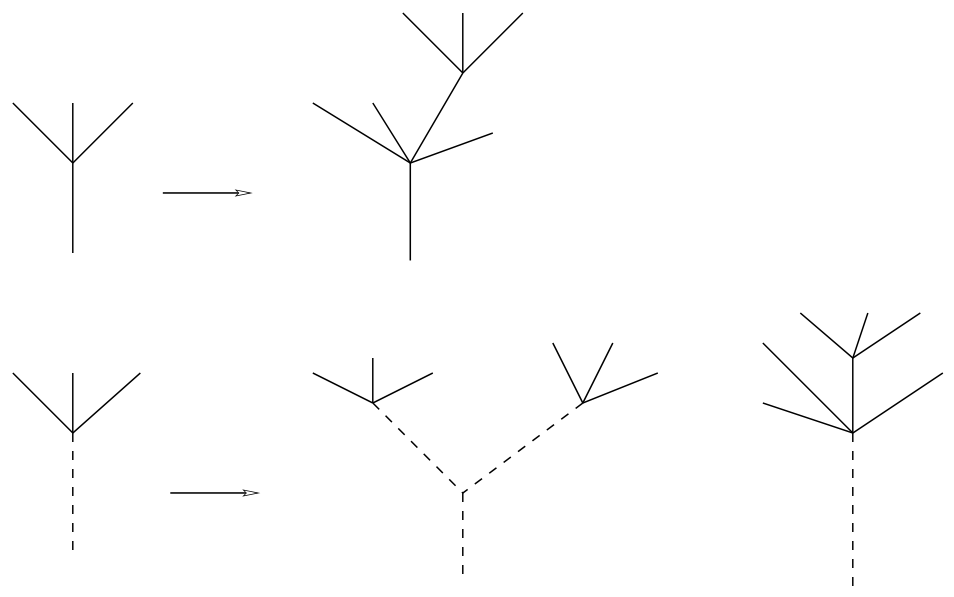
\includegraphics[width=0.6\textwidth]{fig09-ainfty-tree.png}
  \caption{$A_\infty$-关系（上）与 $A_{\infty}$-函子关系（下）是图中右侧所示的一类复合之和（原文 Figure~8，第 25 页）。\label{Fig:Ainftytree}}
\end{figure}

\begin{Remark} \emph{严格幺}的 $A_{\infty}$-范畴 $\scrA$ 是指：对每个对象 $X$ 都有单位元 $e_X \in hom^0_{\scrA}(X,X)$，使得这些 $e_X$ 都是闭的，即 $\mu^1_{\scrA}(e_X)=0$，并且
\[
\mu^2_{\scrA}(a,e_X) = a = (-1)^{|a|}\mu^2_{\scrA}(e_X, a), \quad \mu^k_{\scrA}(\ldots, e_X, \ldots) = 0 \ \forall \, k\geq 3.
\]
若 $H(\scrA)$ 是幺的，即 $H(\scrA)$ 是通常意义下的线性范畴，则称 $\scrA$ 为\emph{上同调幺}的。任何上同调幺的 $A_{\infty}$-范畴都拟同构于一个严格幺的 $A_{\infty}$-范畴 \cite{FCPLT}。
% [Tutor Note: 这里右单位与左单位相差符号：$\mu^2(a,e_X)=a$ 而 $\mu^2(e_X,a)=(-1)^{|a|}a$，这是分次约定下的必然结果；再加上 $\mu^k(\ldots,e_X,\ldots)=0\ (k\geq 3)$ 才得到“严格”单位。对照 §4.3 末可知 Fukaya 范畴一般只在上同调意义下幺。]
\end{Remark}

\subsection{$A_{\infty}$-模与扭曲复形}

$A_{\infty}$-模 $\scrM$ 是范畴 $nu$-$fun(\scrA^{opp},Ch)$ 的一个元素，其中 $Ch$ 是链复形的 $dg$-范畴。具体地说，它给每个 $X\in$ Ob$\,\scrA$ 配备一个 $\bZ$ 或 $\bZ_2$-分次的 $\bK$-向量空间 $\scrM(X)$，并对 $k\geq 1$ 给出映射
\[
\mu_{\scrM}^k: \scrM(X_{k-1}) \otimes hom_{\scrA}(X_{k-2},X_{k-1}) \otimes \cdots \otimes hom_{\scrA}(X_0,X_1) \rightarrow \scrM(X_0)[2-k].
\]
% [Tutor Note: 注意 $\mu_{\scrM}^k$ 的输入次序是模元素打头、态射按“自右向左”排列（$\scrM(X_{k-1})\otimes hom(X_{k-2},X_{k-1})\otimes\cdots$）；这一顺序与 $\mu_{\scrA}^k$ 的输入约定一致，是“从右往左复合”记号的体现，写错次序会直接影响下面的 Yoneda 公式。]
$A_{\infty}$-函子方程蕴含 $\mu_{\scrM}^1$ 是链复形 $\scrM(X_0)$ 上的微分。对任意 $Y \in$ Ob$\,\scrA$，有相应的 \emph{Yoneda} 模 $\scrY$，定义为
\[
\scrY(X) = hom_{\scrA}(X,Y); \quad \mu_{\scrY}^d = \mu_{\scrA}^d.
\]
对应 $Y \mapsto \scrY$ 延拓为一个标准的非幺 $A_{\infty}$-函子 $\scrA \rightarrow mod$-$(\scrA)$，即 Yoneda 嵌入。$A_{\infty}$-模范畴自然是一个\emph{三角}$A_{\infty}$-范畴：态射有锥。更精确地说，若 $c\in hom_{\scrA}(Y_0,Y_1)$ 是次数为零的上循环，即 $\mu^1_{\scrA}(c)=0$，则有 $A_{\infty}$-模 Cone$(c)$，定义为
\begin{equation}\label{eqn:cone}
\mathrm{Cone}(c)(X) = hom_{\scrA}(X,Y_0)[1] \oplus hom_{\scrA}(X,Y_1)
\end{equation}
其运算 $\mu^d_{Cone(c)}((b_0,b_1),a_{d-1},\ldots,a_1)$ 由下面一对项给出
\[
\left(\mu_{\scrA}^d(b_0,a_{d-1},\ldots,a_1), \mu_{\scrA}^d(b_1,,a_{d-1},\ldots,a_1)+ \mu_{\scrA}^{d+1}(c,b_0,a_{d-1},\ldots,a_1) \right).
\]
% [Tutor Note: 原文此处 $\mu_{\scrA}^d(b_1,,a_{d-1},\ldots,a_1)$ 多写了一个逗号（源码笔误），已照抄保留；其含义显然是 $\mu_{\scrA}^d(b_1,a_{d-1},\ldots,a_1)$，请以 PDF 第 26 页为准核对。]
% [Tutor Note: 锥的公式是 Yoneda 模的全忠实性在起作用：$\scrY_0$ 的 $hom(X,Y_0)$ 与 $\scrY_1$ 的 $hom(X,Y_1)$ 直接拼成 $\mathrm{Cone}(c)$ 的两个分量，$c$ 通过 $\mu^{d+1}$ 进入第二个分量的修正项；这正是“锥由态射 $c$ 的一次复合给出”的代数影子。]
% [Tutor Note: $\scrY(X)=hom_{\scrA}(X,Y)$ 关于 $X$ 是反变的，因此 $\scrY$ 是 $A_{\infty}$ 范畴 $\scrA$ 的（右）模，即 $\scrA^{opp}$ 上的函子；而 $\mu_{\scrY}^d=\mu_{\scrA}^d$ 说明 Yoneda 模的结构映射就是原范畴的复合运算，$Y\mapsto\scrY$ 的全忠实性即 $A_\infty$ 版本的 Yoneda 引理。]
可以推广映射锥的构造，考虑 $\scrA$ 中的\emph{扭曲复形}。首先，加性扩张 $\Sigma\scrA$ 的对象是形式直和
\begin{equation} \label{eq:twisted_complex_vector_space}
X = \oplus_{i\in I} V^i \otimes X^i
\end{equation}
其中 $\{X^i\} \in$ Ob$\,\scrA$，$V^i$ 是有限维分次 $\bK$-向量空间。一个扭曲复形是一对 $(X,\delta_X)$，其中 $X \in \Sigma\scrA$，而 $\delta_X \in hom^1_{\Sigma\scrA}(X,X)$ 是微分构成的矩阵
\begin{equation} \label{eq:twisted_complex_differential}
\delta_X = (\delta_X^{ji});\qquad \delta_X^{ji} = \sum_k \phi^{jik} \otimes x^{jik}
\end{equation}
其中 $\phi^{jik} \in Hom_{\bK}(V^i,V^j)$，$x^{jik} \in hom_{\scrA}(X^i,X^j)$，且总次数满足 $|\phi^{jik}| + |x^{jik}| = 1$。微分 $\delta_X$ 应满足两条性质
\begin{itemize}
\item $\delta_X$ 关于 $X$ 的某个滤过是严格下三角的；
\item $\sum_{r=1}^{\infty} \mu^r_{\Sigma\scrA}(\delta_X,\ldots,\delta_X)=0$。
\end{itemize}
% [Tutor Note: 扭曲复形的全部符号约定都浓缩在“$\delta_X\in hom^1$ 且总次数 $|\phi^{jik}|+|x^{jik}|=1$”这两条里：矩阵元按行/列重排或取转置时会额外产生 Koszul 符号，这是计算 $\Tw$ 中态射微分时最常见的错误来源，下文“卷起”公式 \eqref{Eqn:RollTriangle} 正依赖于此约定。]
扭曲复形构成 $A_{\infty}$-范畴 Tw$(\scrA)$ 的对象，其性质是：所有态射都可以通过补上锥而置于正合三角中。而且，正合三角可以被相当有效地操作，例如可以把它们“卷起”：
\begin{equation} \label{Eqn:RollTriangle}
\xymatrix{ X_0 \ar^{a}[r] & X_1 \ar[r] & \ar@/^1.5pc/[ll]_{[1]} Y}, \ 
\xymatrix{ X_1 \ar^{b}[r] & X_2 \ar[r] & \ar@/^1.5pc/[ll]_{[1]} Z} \ \Rightarrow \ 
\xymatrix{ X_0 \ar^{ba}[r] & X_2 \ar[r] & \ar@/^1.5pc/[ll]_{[1]} \mathrm{Cone}(Z\to Y)}
\end{equation}
这意味着也可以操作上同调中相应的长正合列。把对象 $X$ 与置于某个非零次数的 $\bK$ 作张量积，便知 Tw$(\scrA)$ 具有一个\emph{平移函子}，其作用是把所有态射群的次数向下平移一。在 $\bZ_2$-分次情形，该函子的平方是平凡的。

最后，\emph{导出范畴} $D^{\pi}(\scrA) = H(\Tw^{\pi}(\scrA))$ 由如下方式得到：先取 Tw$(\scrA)$ 的幂等完备化——它加入新对象，使得 $H(\Tw\, \scrA)$ 中任何上同调幂等态射在 Tw$^{\pi}(\scrA)$ 中分裂——然后过渡到上同调。它有时也称为\emph{完美模}范畴，记作 Perf$(\scrA)$。尽管构造相当繁复，它却是一个性质良好的 $A_{\infty}$-范畴：由于既三角又幂等完备，它常常能由有限数据（在某个未知拟同构的意义下）重构出来，见第~\ref{Sec:Generation}~节，这是 $\scrA$ 与 Tw$(\scrA)$ 本身都做不到的。

\subsection{全纯多边形}

设 $X$ 是辛流形；为简单起见，我们假定它满足某种恰当性或单调性，并只考虑恰当或单调的拉格朗日，而不去处理障碍理论。我们遵循 \cite{FCPLT, Sheridan3}，通过对 Hamilton 扰动的一致选取来构造 Fukaya 范畴。

首先，固定一族（通常有限）的拉格朗日 $\scrL$，要求它们恰当或单调、可定向且紧致。Fukaya 范畴 $\scrF(X)$ 将是一个 $\bK$-线性的 $A_{\infty}$-范畴，对象为 $\scrL$ 的元素。若 char$(\bK)\neq 2$，我们还假定 $\scrL$ 的元素带有 spin 结构。给定 $\scrL$ 中一对拉格朗日 $(L_0, L_1)$，固定一个紧支的 Hamilton 函数
\begin{equation}
  H_{L_0,L_1} :  [0,1] \times X \rightarrow \bR
\end{equation}
其时间 $1$ 流把 $L_0$ 映为与 $L_1$ 横截的拉格朗日 $\phi_H^1(L_0)$。以 $\Chord(L_0,L_1)$ 记交点集 $\phi_H^1(L_0) \pitchfork L_1$，并令
\begin{equation}
  CF^*(L_0,L_1) \equiv \bigoplus_{x \in \Chord(L_0,L_1)}  \ro_{x}
\end{equation}
其中 $\ro_x$ 是 $x$ 处的 $1$ 维 $\bK$-向量空间，代表“相干定向”，见 \cite[Section 11h]{FCPLT}；它经由 $\overline{\partial}$-算子的指标理论而与 $x$ 相联系。我们取由映射 $J: [0,1] \rightarrow \scrJ$ 给出的时变近复结构，它在区域 $[0,1] \times \bR$ 上定义 $\bR$-平移不变的结构。$CF^*(L_0,L_1)$ 中的微分计数 Floer 轨道，即关于 $J$ 的方程 \eqref{eq:Floer} 的刚性（虚拟维数为零）解。我们假定 $H_{L_0,L_1}$ 与 $J$ 都取一般位置，使这些模空间是正则的，见 \cite{FHS}。

为了在范畴上定义 $A_{\infty}$-结构，对 $k\geq 2$ 以 $\scrR^{k+1}$ 记边界上有 $k+1$ 个穿孔的圆盘模空间；这些区域都是刚性的，其模空间就是 Stasheff 结合面体。以 $\Delta$ 记 $\bC$ 中的单位圆盘。按照 \cite[Section 12g]{FCPLT}，我们通过固定 $p_0$、$p_1$、$p_2$ 的位置来定向 $\scrR^{k+1}$，从而把 $\scrR^{k+1}$ 的内部等同于 $(\partial \Delta)^{k-2}$ 的一个开子集，后者带有标准定向。固定好这个特殊的穿孔 $p_0$ 之后，其余 $\{p_1,\ldots, p_k\}$ 沿边界逆时针排序。沿用 \cite[Section 9g]{FCPLT}，为所有穿孔选取条状端的族。具体地，置
\begin{equation} \label{eqn:in-out-striplike-ends}
  Z_- = (-\infty,0] \times [0,1] \textrm{ and } Z_+ = [0,\infty) \times [0,1]
\end{equation}
并对每个曲面 $\Sigma \in \scrR^{k+1}$ 选取共形嵌入
\begin{equation}
\epsilon_{0}: Z_- \rightarrow \Sigma, \quad \epsilon_i: Z_+ \rightarrow \Sigma \quad  \textrm{for} \, 1 \leq i \leq k\end{equation}
它们把 $\partial Z_{\pm}$ 映入 $\partial \Sigma$，并在端处收敛到穿孔 $p_i$。条状端选取的这一差别反映了如下事实：$p_0$ 将作为 $A_{\infty}$-运算的输出，而其余 $p_i$ 是输入。

给定 $\scrL$ 中对象序列 $(L_0, \ldots, L_k)$，我们接着在 $\scrR^{k+1}$ 上的万有曲线上选取非齐次数据。给定 $\Sigma \in \scrR^{k+1}$ 与 $z \in \Sigma$，该数据包含一个映射
\begin{equation}
  K : T_{z} \Sigma \to C^{\infty}_{ct}(X, \bR)
\end{equation}
并满足约束 $\epsilon_i^* K = H_{L_{i-1},L_{i}} dt$。（空间 $\scrR^{k+1}$ 的 Deligne--Mumford 紧化的边界层是较小结合面体的乘积；非齐次数据在这些模空间上归纳地构造，使之与该分层以及条状端都相容。）$K$ 定义 $\Sigma$ 上一个取值于 $X$ 上向量场空间的 $1$-形式，即 $Y(\xi) = X_{K(\xi)}$（其中 $X_H$ 照例是 $H$ 对应的 Hamilton 向量场）。由此得到 Floer（即扰动 Cauchy--Riemann）方程
\begin{equation} \label{eq:Floer_equation_0-puncture}
 J \left( du(\xi) - Y(\xi)  \right) = du(j \xi) - Y(j \xi) ,
\end{equation}
作用于满足如下条件的映射 $u: \Sigma \to X$ 的空间上：把圆盘上从 $p_{i-1}$ 到 $p_{i}$ 的边界段映入 $L_i$。我们以
\[
  \scrR^{k+1}(X | x_0; x_k ,\cdots, x_1)
\]
记能量有限、且沿端 $\epsilon_i$ 收敛到 $x_i$ 的解空间。标准正则性结果蕴含：对一般数据，该空间是一个光滑流形，其维数为
\begin{equation} \label{Eqn:VirDim}
k - 2 +  \deg(x_0) - \sum_{i=1}^k \deg(x_i).
\end{equation}

Gromov--Floer 构造给出 $  \scrR^{k+1}(X| x_0; x_k ,\cdots, x_1 )  $ 的一个由稳定圆盘组成的紧化。我们施加的恰当性或单调性假设保证：若 $\scrR^{k+1}(X | x_0; x_k ,\cdots, x_1)$ 的维数至多为 1，则紧化中不含球泡或圆盘泡，并且仍是维数正确的光滑闭流形。模空间相对于定向线，由结合面体上所选定的定向而定向。特别地，只要 \eqref{Eqn:VirDim} 为零，对 $  \scrR^{k+1}(X|x_0; x_k, \ldots, x_1) $ 的元素作有符号计数就定义一个映射：
\begin{equation} \label{eqn:summand}
   \ro_{x_k} \otimes  \cdots \otimes \ro_{x_1} \to \ro_{x_0}.  
\end{equation}
按定义，\eqref{eqn:summand} 给出 $A_{\infty}$-运算 $\mu_{\scrF(X)}^k$ 限制在给定输入上的 $\ro_{x_0}$-分量：
\begin{equation}
   \ro_{x_k} \otimes  \cdots \otimes \ro_{x_1}  \subset CF^*(L_{k-1}, L_k) \otimes \cdots \otimes CF^*(L_{0}, L_1)  \to CF^*(L_{0}, L_k).
\end{equation}
$A_{\infty}$-关系是带边界标记点的稳定圆盘模空间之 Deligne--Mumford 紧化 $\overline{\scrR}^{k+1}$ 的代数投影：二次结合性方程中的各项对应于奇异稳定圆盘边界轨迹中的余维一胞腔，参见图~\ref{Fig:DMboundary}（并与图~\ref{Fig:BrokenTriangles} 比较）。下一个紧化 $\overline{\scrR}^{5}$ 是一个五边形，其五个面就是涉及 $\mu^4$ 的第一个二次方程中的各项，等等。
% [Tutor Note: 维数核对：\eqref{Eqn:VirDim} 中的 $k-2$ 正是 $k+1$ 个边界标记点圆盘模空间的维数——扣去三个保角自同构自由度后为 $(k+1)-3=k-2$，恰等于 Stasheff 结合面体的维数；$\overline{\scrR}^{k+1}$ 的余维一界面是若干低维结合面体之积，故 $A_\infty$ 方程的每一项恰对应一个界面。$\overline{\scrR}^4$ 是一维线段，$\overline{\scrR}^5$ 是五边形（五个面 = 含 $\mu^4$ 的方程的五项）。]

\begin{figure}[ht]
  \centering
  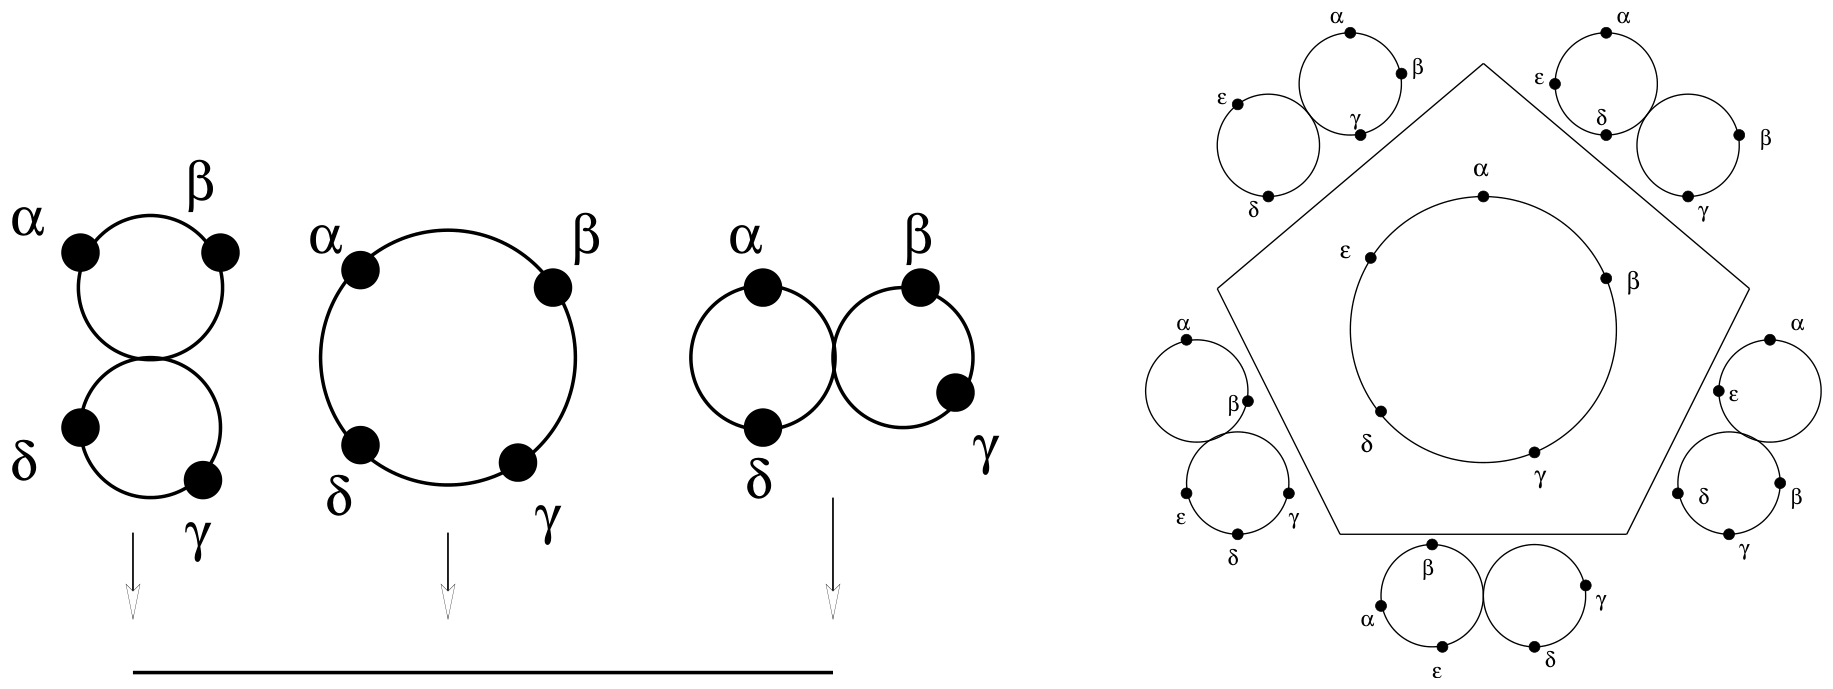
\includegraphics[width=0.95\textwidth]{fig10-dm-boundary.png}
  \caption{紧化 $\overline{\scrR}^4(\delta;\alpha,\beta,\gamma)$ 与 $\overline{\scrR}^5(\epsilon;\alpha,\beta,\gamma,\delta)$（原文 Figure~9，第 28 页）。\label{Fig:DMboundary}}
\end{figure}

\begin{Example} \label{Ex:CoveringSpace} Fukaya 范畴由全纯圆盘搭成，而全纯圆盘可以提升到覆叠空间。
设 $\pi:\tilde{M} \rightarrow M$ 是 Stein 流形的有限 Galois 覆叠，并以 $\scrF(\cdot)$ 记恰当 Fukaya 范畴。存在一个函子
$\pi^*: \scrF(M) \longrightarrow \scrF(\tilde{M})$，
它把 $L \in \scrF(M)$ 送到完全原像 $\pi^{-1}(L) \subset \tilde{M}$，并且态射上的映射 $HF^{*}(L,L) \to HF^{*}(\pi^{-1}(L), \pi^{-1}(L) )$
与经典的上同调拉回一致（由于群作用的不动点集假定为平凡，等变横截性不成问题）。$\pi$ 的覆叠变换通过 $\scrF(\tilde{M})$ 的自等价而作用。
\end{Example}

Fukaya 范畴是上同调幺的，因为 $HF^*(L,L)$ 是幺环。然而它们并非“几何地”严格幺，即通常不存在严格的单位元，除非施加某种抽象的拟同构。

% [Tutor Note: “上同调幺”与“几何严格幺”的区分值得留意：$[e_L]\in HF^*(L,L)$ 是幺元，但 $CF^*(L,L)$ 上通常没有严格单位元，必须先作抽象的拟同构才能得到严格幺模型；这正是 $A_\infty$ 范畴中“单位”只能在同伦意义下谈论的原因。]
在少数情形，可以把从扭曲复形 $\Tw\,\scrF(X)$ 到其幂等完备化 $\Tw^{\pi}\scrF(X)$ 的过渡理解如下：迭代的 Lagrange 手术（我们期望把它解释为映射锥）产生可能不连通的拉格朗日子流形，而取分裂闭包时就把各个连通分支都包括进来。一般并没有这样的几何解释：例如对于对角 $S^2 \subset \bP^1\times(\bP^1)^-$，Floer 上同调 $\cong QH^*(\bP^1)$ 有幂等元，而该对象的分裂项的同调类是 $(1\pm[S^2])/2$，并不落在纯次数上。

\subsection{扭转}

一类特别重要的映射锥来自扭转函子。给定 $Y \in$ Ob$\,\scrA$ 与一个 $\scrA$-模 $\scrM$，定义\emph{扭转} $\scrT_Y\scrM$ 为模
\[
\scrT_Y\scrM(X) = \scrM(Y)\otimes hom_{\scrA}(X,Y)[1] \oplus \scrM(X)
\]
它正是标准求值态射
\begin{equation} \label{Eqn:Twist}
\scrM(Y) \otimes \scrY \rightarrow \scrM,
\end{equation}
之上的锥，其中 $\scrY$ 表示 $Y$ 的 Yoneda 像。对两个对象 $Y_0, Y_1 \in$ Ob$\, \scrA$，扭转的本质特征是它在 $H(\scrA)$ 中给出一个标准的正合三角
\[
\cdots \rightarrow Hom_{H(\scrA)}(Y_0,Y_1) \otimes Y_0 \rightarrow Y_1 \rightarrow T_{Y_0}(Y_1) \stackrel{[1]}{\rightarrow} \cdots
\]
其中 $T_{Y_0}(Y_1)$ 是任一 Yoneda 像为 $\scrT_{Y_0}(\scrY_1)$ 的对象；若 $H(\scrA)$ 的态射空间有限维，这样的对象必然存在，参见 \cite[p. 64]{FCPLT}。
% [Tutor Note: 扭转公式 $\scrM(Y)\otimes hom(X,Y)[1]\oplus\scrM(X)$ 就是求值态射 $\scrM(Y)\otimes\scrY\to\scrM$ 的锥（$\scrY$ 的 Yoneda 像贡献出 $hom(X,Y)$）；因此“扭转 = 沿 Yoneda 模的锥”是 $A_\infty$-模层面的构造，而几何上的正 Dehn 扭转 $\tau_L$ 是 $\scrF(X)$ 的自等价——Seidel 定理断言二者在球面 $L$ 上拟同构，这把代数锥与 Lagrange 手术的映射锥对应起来。]

对 Fukaya 范畴，当 $L$ 为\emph{球面}的，即 $\Hom_{\mathrm{Don}(X)}(L,L) \cong H^*(S^n)$ 时，扭转函子 $\scrT_L \in nu$-$fun(\scrF(X),\scrF(X))$ 起着特殊的作用。设 $L\subset X$ 是拉格朗日球面；\emph{几何扭转} $\tau_L$ 是由 $L$ 中的正 Dehn 扭转所定义的 $\scrF(X)$ 的自等价，参见第~\ref{Sec:Appl1}~节。
另一方面，在单调或恰当情形，这样的球面给出 Fukaya 范畴 $\scrF(X)$ 的一个良好定义的对象（尽管在单调情形\emph{先验地}未必非零），从而给出上面所述的代数扭转函子。

\begin{Theorem}[Seidel] \label{Prop:twists}
若 $L\subset X$ 是拉格朗日球面，并在 $L \cong S^1$ 时带有非平凡的 \emph{Spin} 结构，则 $\tau_L$ 与 $\scrT_L$ 在 $nu$-$fun(\scrF(X),\scrF(X))$ 中拟同构。
\end{Theorem}
% [Tutor Note: 证明见 \cite[Corollary 17.17]{FCPLT}：其核心是把正 Dehn 扭转沿球面 $L$ 分解为“粘接”操作，再与 $HF^*(L,L)\cong H^*(S^n)$ 的代数数据逐项比对；注意 $L\cong S^1$ 时必须取非平凡 Spin 结构，否则定向线上差一个符号，结论会差一个平移。]

这就是 \cite[Corollary 17.17]{FCPLT} 在恰当辛流形情形下的结论，单调情形的论证类似。它给出了代数与几何之间的一个基本联系，并强化了我们此前在第~\ref{Subsec:ExactTriDon}~节中引入的 Donaldson 范畴中的正合三角。
